%%%%%%%%%%%%%%%%%%%%%%%%%%%%%%%%%%%%
%%%%%%%%%%%%%%%%%%%%%%%%%%%%%%%%%%%%
%%%%%%%%%%%%%%%%%%%%%%%%%%%%%%%%%%%%
\section{General Semistructured Query Language (GSQL)}\label{sec:gsqldef}
As  observed within the dynamic graph context \cite{Demetrescu2010}, the four main unary graph operations that a database must support are the insertion,  deletion, and the update of the basic components of a data structure, alongside with its navigation (filtering). Please note that, within  (nested) graphs, the vertices' and edges' operations must be implemented differently: while the removal of an edge has no consistency problems, the removal of a vertex must imply the removal of all the incoming and outgoing edges and, in this sense, it can be considered as the removal of several elements at once. This observation leads to the fact that we can't unify one same operator for different data constructors. Therefore, we only way to generalise such operations is to generalise and de-specialise the data model, as it has been already done for GSM. Moreover, the graph join contribution in Chapter \ref{cha:join} also showed that binary graph operations can be all implemented with the same subset of relational operations plus some refinements required to preserve the data model's constraints (see Section \vref{ssec:ngrahop}). This intuition can be supported by the GSM model, where both vertices and edges are represented as objects: %, having different containment expressions and labels. 
for example, instead of defining an explicit operation allowing the creation of new edges, we can  define an operation creating new objects within the GSM that is also going to be used for the edge creation task. By doing so, the object creation operation may be also used in further several data representations, from relational data, to semistructured and nested graphs as represented in GSM. Given that also different models and operations may come after this thesis, we want to provide the most basic set of operations that may be adopted  as a common basis by either current or subsequent query languages over GSM. 

Before providing a definition for nested graphs, we're going to describe the basic operations to be used within the nested semistructured model. \marginpar{\textit{Object Creation}$\rhd$ }We're now going to discuss and motivate the object creation operator: this operation is generally required by our data model, because such model can only express $\phi$ containment over objects that already exist. Therefore, if we want either to extend  or aggregate some objects, we must create first an object representing either its extension or  aggregation. The object creation operator can be defined as follows:

\begin{definition}[Object Creation]\label{gsql:objcreate}
	Given an GSM $n=(o,O,\ell,\xi,\phi)$, \index{GSQL!$\texttt{create}$} the \textbf{object creation} of $\omega\notin O$ associated to a set of labels $L$ and expressions $E$ with a containment function $\phi_\omega$ for a list of elements already contained in $O$ ($\cod(\phi_\omega)\subseteq \partof{O}$) is defined as follows:
	\[\texttt{create}^\omega_{L,E,\phi_\omega}(n)=(o_c,O\cup\{\omega\},\ell\oplus[[\omega, L]],\xi\oplus[[\omega, E]],\phi\oplus[[\omega,\phi_\omega]])\]
\end{definition}

 In particular, both ontology alignments and data cleaning processes \cite{ALIEH17} use the creation of new relationships for storing the similarity between the matched values; such operation is called \textbf{link discovery} or \textbf{match} (see Section \vref{ssec:ngrahop}).

The removal of an element from an object (or a collection) is not a primitive operation,\marginpar{$\lhd$ \textit{Object removal is a specific case of filtering}} because it can be expressed through a filtering predicate expressing the concept ``not appearing in''. In particular, within the relational model we can express a set difference $A\backslash B$ (stating the removal from $A$ of all the objects contained by $B$) through a selection predicate as follows:
\begin{equation}\label{eq:difference}
A\backslash B = \Set{x\in A | x\notin B}=\sigma_{x\mapsto x\notin B}(A)
\end{equation}
Moreover, the  database filtering\footnote{Within the context of relational algebra, such operation is referred as \textit{selection} ($\sigma$). The term filtering is here used instead of select, because the latter one has a completely different meaning in other query languages, such as SQL, where its remarks a projection operation.} is the most relevant operation for several traversal and visiting tasks \cite{ThakkarPAV17,Neo4jAlg,MartonSV17,NautiLOD}. \marginpar{$\lhd$ \textit{Filtering is a specific case of mapping}}Nevertheless, the filtering operation can be further on generalized by the definition of a transformation function: given that all the GSM objects can contain  other objects associated to properties within $\phi$, it implies that the filtering operation over the objects has to be considered as a special case of the ``update'' or map operation, where the non-desired objects may also be removed. \marginpar{$\lhd$\textit{Map operator}.} Let us define the map operator first, which will update any object $o_c$ contained in the object repository $O$ by creating a new one with a different id ($o_{c+1}$) when at least one of his two functions are not involve into a transformation:

\begin{definition}[Map]\label{gsql:map}
	Given an GSM $n=(o,O,\ell,\xi,\phi)$, the \textbf{map}\index{GSQL!$\texttt{map}$} operator $\texttt{map}_{f_L,f_E,f_C}$ associates to each object $o$ represented in $\varphi^*(o)$, $o$ included, a new one having labels $f_L(o)$, expressions $f_E(o)$ and containments $f_C(o)$. Moreover, it associates a new id to all the transformed objects $\delta O$ such that $\delta O=\Set{o\in O|f_L(o)\neq \ell(o)\vee f_E(o)\neq \xi(o)\vee f_C(o)\neq \phi(o)}$:
	\begin{alignat*}{3}
	\texttt{map}_{f_L,f_E,f_C}(n)=(&o &&{}_{c+1},\\
	&O&&\cup[o {}_{c+1}|o_c\in \delta O],\\
	&\ell&&\oplus \bigoplus_{o_c\in \delta O} [[o_{c+1},\; f_L(o_c)]],\\
	&\xi&&\oplus \bigoplus_{o_c\in \delta O} [[o_{c+1},\;  f_E(o_c)]],\\
	&\phi&&\oplus \bigoplus_{\substack{o_c\in \delta O}}  [[o_{c+1},\; \bigoplus_{e\in\dom(f_C(o_c))} [[e,\; [o'_{c+1}|o'_c\in f_C(o_c,e)\cap\delta O]\cup(f_C(o_c,e)\backslash \delta O)]]]] \\
	&)\\
	\end{alignat*}
	Please note that the double-squared ``graph of a function'' notation introduced ad page \pageref{def:doublesquarednotation} is used to describe the functions' updates. Furthermore, if $f_L$ is defined using \texttt{script} programs ($f_L\equiv\jsem{\texttt{expr}}_\Gamma$), the writing $f_L(o_c)$ has to be intended as the evaluation of the associated expression \texttt{expr} where \texttt{o} is associated to $o_c$ and \texttt{g} to $o_c$ ($f_L(o_c)\eqdef \jsem{\texttt{expr}}_{\Gamma\cup\{(\texttt{o},o_c),(\texttt{g},o)\}}$). Similar considerations can be also carried out for $f_E$ and $f_C$. Last, the user must be aware that this operation may transform a nesting-loop free GSM into a general GSM due to the arbitrary way of performing nestings.
	%Please note that if the map function must not apply one of the three transformation functions or even just a partial transformation is performed, a placeholder $\cdot$ can be put. E.g.:
	%\[\texttt{map}_{\cdot\oplus[o_c\mapsto \{L\}],\cdot,\cdot}(n)=\texttt{map}_{\ell\oplus[o_c\mapsto \{L\}],\xi\,\phi}(n)\]
\end{definition}
%Please also note that a map operation cannot be expressed by solely iterating the creation over the updated objects $\delta O$, because it must also involve the update of the containment functions, that cannot be expressed by a simple creation operation.
We can now express a filtering operator using \texttt{map}: given a GSM $n=(o,O,\ell,\xi,\phi)$,
the selection of the objects upon a predicate $P$ within an object containment is expressed by the \texttt{map} operator:
\begin{equation}\label{eq:selection}
\texttt{filter}_P(n)\eqdef \texttt{map}_{\jsem{\texttt{o.\textbf{ell}}}_\Gamma,\jsem{\texttt{o.\textbf{xi}}}_\Gamma,\jsem{\scriptline{map((o.phi) : x -> { [x[0], select(x[1] : P)]})}}_\Gamma}(n)
\end{equation}
where each expression is going to be evaluated with a context $\Gamma$ where $o$ is associated to the currently evaluated object and $g$ is $n$.

These two operators will permit the implementation of most of the unary operators. In order to increase the operations that our language is able to express, we must also include the $n$-ary operators, taking more than just one data input. \marginpar{\textit{(S)electing the $\rhd$ object over which perform the operations}.} Before defining such operator, we must be able to select one specific object within the GSM, over which we're going to perform the $n$-ary operations in a subsequent step. Most graph  and relational $n$-ary operations are applied within the same database, where we often have to select the operands over which the queries have to be carried out: (e.g. \texttt{FROM} in SQL, \texttt{GRAPH} in SPARQL). The selection may be implemented by changing (e.g., ``electing'') the reference object for the current GSM. Therefore, this preliminary election operator for $n$-ary operations is defined as follows:

\begin{definition}[Elect]\label{gsql:elect}
Given an GSM $n=(o,O,\ell,\xi,\phi)$, \index{GSQL!$\texttt{elect}$} the \texttt{elect} operation chooses an object $o'\in O$ to be used as a new object reference for GSM.
\[\texttt{elect}_{o'}(n)=(o',O,\ell,\xi,\phi)\]
\end{definition}

\begin{figure}[!t]
	\centering
  \begin{minipage}[t]{0.9\textwidth}
	 \centering
	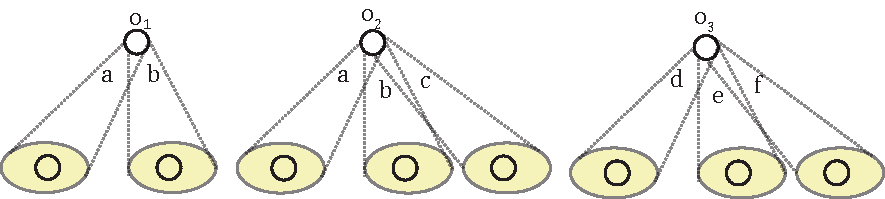
\includegraphics[scale=0.8]{fig/05language/01disjoint_input.pdf}
	\subcaption{$n$ possible operands for the \texttt{disjoint} operator. In particular, each object $o_i$ is the reference object for the GSM $n^i$.}
	\label{fig:disjoperands}
\end{minipage}
\begin{minipage}[t]{0.6\textwidth}
	\centering
	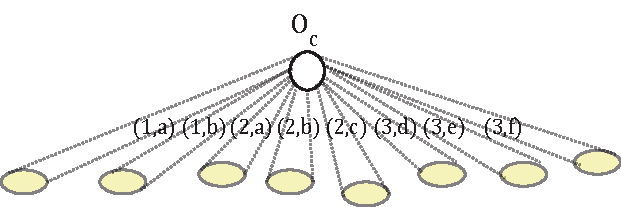
\includegraphics[scale=0.8]{fig/05language/02disjoint_output.pdf}
	\subcaption{Result of  $\texttt{disjoint}(n^1,n^2,n^3)$.}
	\label{fig:disjsol}
\end{minipage}
\caption{\texttt{disjoint} operator. As you can see from the picture, each collection from the operand $o_i$ is treated as a separate element of o and, consequently, mapped into the final result $o_c$.}
\label{fig:disjoint}
\end{figure}

After providing the possibility of electing the GSM's references, we can now define the class of all the non-recursive $n$-ary operations over GSMs \marginpar{ \textit{$n$-ary disjoint $\rhd$ union operator}}. By taking take $n$ GSMs as inputs, and then mapping  their reference objects into one single object, ${\omega}$, such object is going to have the labels' (and the expression') set as the union of the input reference objects' labels (and expressions') set; the $\phi$ containment expresses the disjoint concatenation of the incoming objects concatenation, such that $\phi(\omega,[i,l]):=\phi(o_c^i,l)$ for each input reference object $o_c^i$ with $1\leq i\leq n$. As a last step, the result of the disjoint union can be mapped as we please to implement the desired $n$-ary operator. Before doing so in the following section, we provide a definition of such operation:

\begin{definition}[$n$-ary Disjoint Union]\label{gsql:disjoint}
	Given $n$ GSMs, (for each $1\leq i\leq n$, $n_i=(o_c^i,O^i,\ell^i,\xi^i,\phi^i)$) their \textbf{$n$-ary disjoint union} \index{GSQL!$\texttt{disjoint}$} $\texttt{disjoint}(n_1,\dots,n_n)$ is defined as the new object having as reference a new object $\omega\notin \bigcup_i O_i$. If the $\omega$ is omitted, then it is generated as  $(\max(\overline{o}^1,\dots,\overline{o}^n)+1)_{max(c^1,\dots,c^n)+1}$, where $\overline{o}^i_{c^i}=\max O^i$ for each $1\leq i\leq n$.
	 The labels (and expressions) associated to $\omega$ are the union of the labels (and expressions) associated to all the reference objects, while the collections are also merged by extending the $\phi^i$  functions.%\footnote{The blue expression expressed in a ``graph of a function'' notation, compatible with \texttt{script}, can be represented by the following function: \[o\mapsto p\mapsto \begin{cases}
			%\phi(o,p') & o \equiv\tilde{o}_c,  p\equiv \Braket{1,p'}\\
%			\phi'(o',p') & o \equiv\tilde{o}_c, p\equiv\Braket{2,p'}\\
%			\end{cases}\]}.
%$\psi_1$ function, which is defined as follows:
%
	The resulting GSM is defined as follows:
	\begin{alignat*}{2}
	\texttt{disjoint}^\omega(n^1,\dots,n^n)=(&\omega,\\
	&\bigcup_{1\leq i\leq n}O^i\;\cup\;\{\omega\},\\
	&\bigoplus_{1\leq i\leq n}\ell^i\;\oplus\;[[\omega,\; \bigcup_{1\leq i\leq n}\ell^i(o_c^i)]]\\
	&\bigoplus_{1\leq i\leq n}\xi^i\;\oplus\;[[\omega\; \bigcup_{1\leq i\leq n}\xi^i(o_c^i)]]\\
	&\bigoplus_{1\leq i\leq n}\phi^i\;\oplus\; {\color{blue}[[\omega,\; \bigoplus_{1\leq i\leq n}\bigoplus_{p\in\dom(\phi(o^i_c))}[[[i,p],\; \phi(o^i_c,p)]]]]})\\
	\end{alignat*}
Later on, we're going to denote $\ell_{n^1,\dots,n^n}$, $\xi_{n^1,\dots,n^n}$ and $\phi_{n_1,\dots,n^n}$ respectively the $\ell$, $\xi$ and $\phi$ functions associated to the GSM resulting from $\texttt{disjoint}^\omega(n^1,\dots,n^n)$.
\end{definition}



\begin{example}
	Figure \vref{fig:disjoint} provides an example of how the disjoint union behaves on three distinct data inputs: as we can see, each collection $\phi(o_i,p)$ belonging to the $i$-th operand is mapped into the collection $\phi(o_c,[i,p])$ of the expected result. This operator allows to keep distinct collections coming from different operands into one single object, and preserves both the operator and the expression from which it comes from.
\end{example}

 We have to define an iterative operator similarly to the \marginpar{$\lhd$ Expressing iterations.} one defined in \cite{Calders2006,apacheflink}:  most data mining algorithms can be expressed as fold operators jointly with the body of the iteration expressed through a GSQL expression, as already introduced in Section \vref{subsec:dmalgebra}. Given that our query language shall not be able to diverge, we will restrict such operator to a finite recursion. In particular, we're going to use the following  high order $\texttt{fold}$ operator that can be applied to any kind of collection.

\begin{definition}[High Order Fold Operator]\label{def:fold}\index{GSQL!fold}
	Given any finite collection $S$ of elements, the $\texttt{fold}$\index{GSQL!\texttt{fold}} operator takes as inputs a collection $S$ of elements of type $\Sigma$ over which the iteration is performed, an accumulator ``$\alpha \colon A$'' providing the initial value, and a binary function $f:\Sigma\to A\to A$. Starting from the min of $S$ $\min(S)$ (e.g., the first element of a collection), $\texttt{fold}$ updates $\alpha$ via $f$  to $f(\min(S),\alpha)$, and then iterates the process until all the elements of $S$ are visited. The final value of $\alpha$ is then returned.
	This function can be recursively written as follows:
	\[\texttt{fold}_{S,f}(\alpha)=\begin{cases}
	\alpha & S=\emptyset\\
	\textup{fold}_{S\backslash\min(S),f}(f(\min(S),\alpha)) & oth.
	\end{cases}\]
	Please note that if $\alpha$ is a GSM, $f$ can be even an arbitrary GSQL expression, and hence it can be used for GSQL expressions. Also note that $S$ can be also a nested graph and, in this case, the iteration is performed over the collection of objects of both vertex and edge set, thus providing another nested graph binary operator.
\end{definition}

 Last, GSQL may also support the creation of view by associating \marginpar{ Views $\rhd$} a variable to a GSQL expression. This concept is widely supported on both relational \cite{Calders2006,atzeniEN,atzeniIT} and graph algebras \cite{GRAD}, in order to be later used as other data inputs. We  formally define a GSQL expression as follows:

\begin{definition}[GSQL expression]
\index{GSQL|textbf}
Given the set  $\mathcal{GSM}$ containing all the possible GSM $n$ and a set $\textup{Var}$ of all the possible variables $V_i$, a GSQL expression \texttt{<GSQL>} is defined as follows:
\[\begin{split}
\texttt{<GSQL>}:&=n\in\mathcal{GSM}\;|\;V\in\textup{Var}\\
	&|\;\texttt{create}^\omega_{L,E,\phi_\omega}(\texttt{<GSQL>})\;|\;\texttt{map}_{f_L,f_E,f_C}(\texttt{<GSQL>})\;|\;\texttt{elect}_o(\texttt{<GSQL>})\\
	&|\;\texttt{disjoint}^\omega(\texttt{<GSQL>}(,\texttt{<GSQL>})^*)\;|\;\texttt{fold}_{S,f}(\texttt{<GSQL>})\\
\end{split}\]
The semantics associated to the evaluation of a GSQL expression was provided\footnote{See also \url{https://bitbucket.org/unibogb/gsql-script/src/f903ff35f16ce2ec6b64bf3a87d68e84e14897e8/src/main/java/it/giacomobergami/nestedmodel2/model/languages/GSQL/?at=master} for its implementation.} by the previous operators' definitions (Definitions \ref{gsql:objcreate}-\ref{def:fold}). The variable's semantics is defined by the evaluation of the associated GSQL expression, if any.
\end{definition}
